\subsection*{Introduction}

    The Performance Profile of a solver is the cumulative distribution
    function of a performance metric, e.g., CPU time, number of functions
    evaluations, number of iterations, or others, that we will call \emph{cost}.

    It was first described by \textcite{Dolan:2002du} and is presented as a 
    graphic that shows the relative performance profile of different solvers, 
    according to a chosen metric, for a given set of problem instances.

    Given a set $\Pset$ of problems and a set $\Sset$ of solvers, for each 
    problem $p \in \Pset$ and solver $s \in \Sset$, we define $t_{ps}$ as the  
    cost required to solve problem $p$ by solver $s$ and
    \begin{align*}
      r_{ps} = \frac{t_{ps}}{\min\{t_{ps}: s \in \Sset\}}
    \end{align*}
    as the performance ratio of solver $s$ for the problem $p$ when compared
    with the best performance by any solver on this problem.

    \citeauthor{Dolan:2002du} define the probability of a solver $s \in \Sset$ to
    solve one problem within a factor $\tau \in \mathds{R}$ of the best
    performance ratio as the function
    \begin{align*}
      \rho_s(\tau) = \frac{| \{p \in \Pset: r_{ps} \leq \tau\} |}{| \Pset |}
    \end{align*}
    For a given $\tau$, the best solver is the one with the highest value for
    $\rho_s(\tau)$.

\subsection*{Motivation}

    To facilitate the reproduction of data set analysis, such as the
    benchmarking of solvers analysis provided by \citeauthor{Dolan:2002du}'s
    performance profile, it is important to have an open source tool that handle
    the production of plots.

    Performance profile has been, over the years, the most used benchmark
    comparison tool used in optimization. Nevertheless, the production of such
    analysis is sometimes a task that can lead a researcher to waste a lot of
    time and effort that should have been spent in developing the solver itself,
    and not in creating the comparison plots. The main goal of our work was to
    create  a straightforward  tool that would allow one to create performance
    profile pictures in a fast and easy manner.

    Moreover,  we wanted to allow \LaTeX\ users, a group in which almost all
    optimization community is included,  to   generate performance profile plots
    within \LaTeX\ environment, and thus to get a better typographic result other
    than simple including raster  images.

    With these two main goals in mind, we developed and implemented perprof-py
    in python3 with internationalization features and direct \LaTeX\ integration.

\subsection*{Implementation and architecture}

    The software was implemented as a Python 3 package, to allow users to work
    internally on the code. This allows, for instance, the creation of a GUI
    as a different software. We also created a command line interface to use the
    software.

    The implementation is very straight forward:
    \begin{enumerate}
      \item First the parse the options passed as arguments, creating a
        structure with all that information;
      \item We then parse and process the input files, using the definition
        of the performance function to create the data to be plotted;
      \item We then use the desired backend to plot the data.
    \end{enumerate}

\subsection*{Input}

    Each solver to be used in the benchmark must have a file like:

    \begin{verbatim}
---
YAML information
---
Problem01 exit01 time01
Problem02 exit02 time02
    \end{verbatim}

    In the YAML information you can set the name of the solver, and some
    flags for perprof-py.
    Each line beyond that has 3 columns that mean, in order:
    \begin{itemize}
      \item The name of the problem;
      \item Exit flag;
      \item Cost measure, such as elapsed time.
    \end{itemize}

\subsection*{Parsing process and output}

    To use perprof-py, the user needs to issue a command of the type
\begin{verbatim}
$ perprof OPTIONS BACKEND FILES
\end{verbatim}
    where
    \begin{itemize}
      \item FILES are the input files described in the previous section, and at
        least two files are required;
      \item BACKEND is one of the options \verb+--tikz+, \verb+--mp+ or
        \verb+--raw+, which represents whether the user wants to use
        Tikz/Pgfplots, MatplotLib or simply printing the performance ratios,
        respectivly;
      \item OPTIONS are varied arguments that can be passed to perprof to
        customize the graphics, or modify the performance functions. Some
        noteworthy options are
        \begin{itemize}
          \item \verb+--semilog+: use a logarithmic scale for the abscissa;
          \item \verb+--success STR+: \verb+STR+ is a comma separated string
            of keys to be considered as success by the algorithm;
          \item \verb+--black-and-white+: differentiate the plots using only
            line styles, and paint them in black;
          \item \verb+--subset FILE+: consider only the problems in the file
            \verb+FILE+ when creating the performance functions.
        \end{itemize}
    \end{itemize}
    The Figures \ref{fig:example1}-\ref{fig:example4} show some examples of the
    performance profile graphics.
    \begin{figure}[!ht]
      \centering
      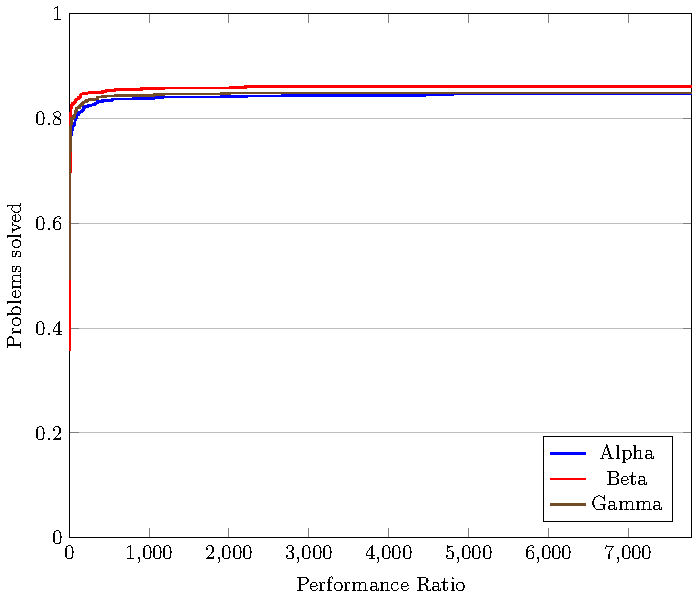
\includegraphics[width=0.4\textwidth]{plots/abc.pdf}
      \caption{Example of performance profile with default options.}
      \label{fig:example1}
    \end{figure}
    \begin{figure}[!ht]
      \centering
      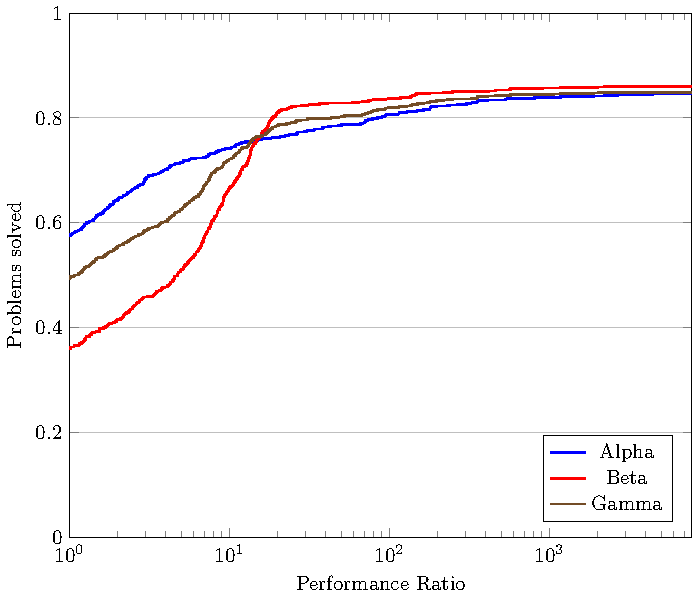
\includegraphics[width=0.4\textwidth]{plots/abc-semilog.pdf}
      \caption{Example of performance profile with semilog option.}
      \label{fig:example2}
    \end{figure}
    \begin{figure}[!ht]
      \centering
      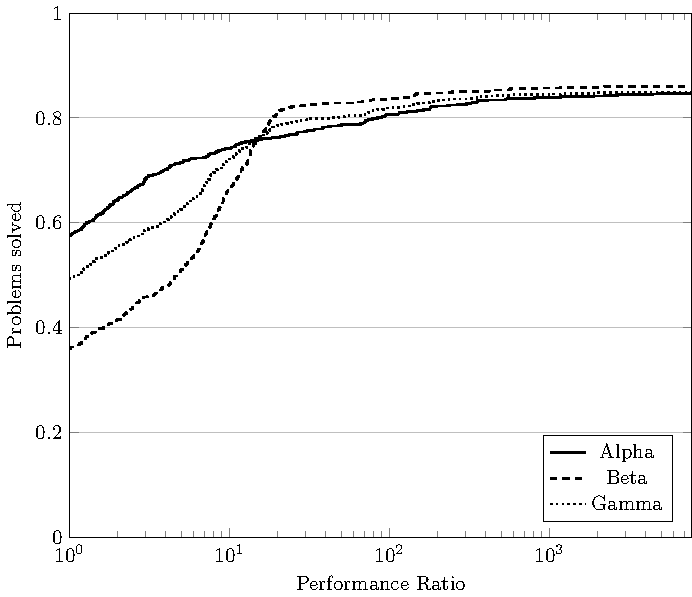
\includegraphics[width=0.4\textwidth]{plots/abc-semilog-bw.pdf}
      \caption{Example of performance profile with semilog and black and white
        options.}
      \label{fig:example3}
    \end{figure}
    \begin{figure}[!ht]
      \centering
      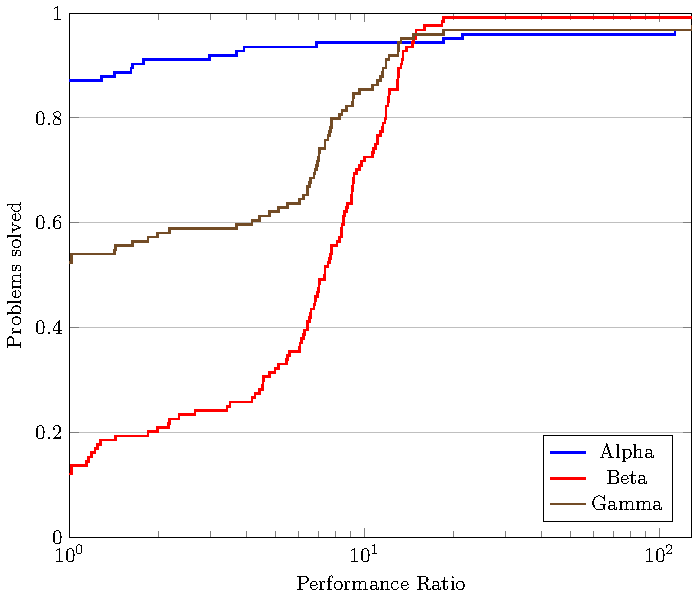
\includegraphics[width=0.4\textwidth]{plots/abc-semilog-hs.pdf}
      \caption{Example of performance profile with semilog and subset options.}
      \label{fig:example4}
    \end{figure}

\subsection*{Quality control}

    The code is tested using unit tests that verify if wrong input information
    is captured. These tests are run automatically on Travis CI
    \cite{url:travis}, for python 3.3 and 3.4.
    In addition, we verified on the stable releases that the code generates the
    desired graphics. This part of the testing must be manual.

